% !TEX root =  ../main.tex
\chapter{Synthèse d'un régulateur discret}

\section{Introduction}
Durant la troisième et dernière séance de laboratoire, il a été demandé aux élèves de synthétiser sur le logiciel MATLAB\textregistered{} un régulateur discret de compensation en boucle fermée et d'en analyser la réponse.
Pour ce faire, il a tout d'abord fallu calculer l'équivalent échantillonné bloqué de ce régulateur (discrétisation).
Et ensuite, imposer un intégrateur dans le régulateur discret de compensation.

\section{Hypothèses}
Soit le système défini par l'équation :
\begin{equation}
	H_c(s) = \frac{1}{s\left( s+0,5\right)}
		   = \frac{2}{s\left(2s+1  \right)}
	\label{eqn:system3}
\end{equation}
Nous cherchons à effectuer la synthèse d'un régulateur discret compensant le système~(\ref{eqn:system3}) en boucle fermée, et respectant les spécifications suivantes :
\begin{enumerate}
	\item Dépassement de 5\% $(\xi=0,69)$
	\item Temps de réponse à 95\% ($3T$) de 1
	\item Erreur de vitesse nulle
	\item $h = 0,1$
\end{enumerate}
Notons avant tout que la spécification sur l'erreur de vitesse nulle implique un double intégrateur dans la chaîne directe.
Ceci nous indique d'avance que le régulateur suivra la forme :
\begin{equation}
	R(Z) = \frac{\dots}{(Z-\alpha)(Z-\beta)}
\end{equation}

%%%%%%%%%%%%%%%%%
\section{Analyse}
La première étape est toujours la même, nous devons traduire la fonction de transfert dans le domaine discret.
Pour cela nous utilisons la commande \texttt{c2d()} de MATLAB\textregistered{} qui équivaut à convoluer la fonction par un bloqueur d'ordre 1.
C.-à-d. effectuer l'opération :
\begin{align}
	H_d(Z) &= \underset{s\rightarrow Z}{\mathcal{L}} H_c(s) \\[2mm]
		   &= \frac{k}{(Z-1)(Z-p)}
		   \label{eqn:uncompensated}
\end{align}
Dans cette forme, les points sont distants de la période d'échantillonnage.
Cela entraine que l'influence de l'entrée sur la sortie est perçue après cette même période.
Ceci implique également que la différence entre l'ordre du dénominateur et du numérateur doit être égale à 1.
Pour imposer cet ordre, nous rajoutons un zéro au numérateur de~(\ref{eqn:uncompensated}).
Ce qui donne :
\begin{equation}
	H_d(Z) = \frac{k\,(Z-z)}{(Z-1)(Z-p)}
\end{equation}

De cette forme discrétisée, nous désirons extraire les pôles et les zéros.
MATLAB\textregistered{} propose une fonction permettant de les extraire en un appel, \texttt{zpkdata()}.
Nous employons par la suite ces coefficients obtenus dans le régulateur $R(Z)$ pour compenser $H_d(Z)$.
$R(Z)$ est donc une régulateur de compensation.

\begin{equation}
	R(Z) = k\,\frac{(Z-p)}{(Z-z)(Z-1)}
\end{equation}
On a un décalage car l'ordre du dénominateur est plus grand que l'ordre du numérateur.
Quand le régulateur aperçoit un écart de réglage à sa consigne, il doit réagir immédiatement.
Il \og{}mouline\fg{} dans un temps qui est supposé très petit et négligeable sur la période puis il envoie.
On rajoute un zéro au numérateur pour faire en sorte qu'il n'y ait pas de retard dans le régulateur.
\begin{equation}
	R(Z) = k\,\frac{(Z-p)(Z-n)}{(Z-z)(Z-1)}
\end{equation}
Ensuite nous faisons le produit en boucle ouverte du régulateur avec le système.
\begin{equation}
	R(Z)H_d(Z) = B_0(Z) = \frac{k\,(Z-n)}{(Z-1)^2}
\end{equation}
On constate que dans le chaîne directe, il y a bien un retard d'une période.

%%%%%%%%%%%%%%%%%%
\section{Synthèse}

Dans le plan complexe les pôles continus sont sur une droite d'amortissement inclinée d'un certain angle \Theta{}, tel que dans notre cas $sin(\Theta) = 0,69$.
C'est le sin de l'angle d'inclinaison de la droite d'amortissement sur laquelle se trouvent les pôles.
Le $sin(\Theta)$ détermine ainsi le dépassement de 5\% cité dans l'énoncé du laboratoire et qui est une des spécifications du régulateur.

Ensuite, nous avons le temps de réponse à 95\% de 1.
Si nous traduisons cela sous forme de pôles et de zéro dans le cas d'un filtre du 1\up{er} ordre, nous trouvons que le lien entre un pôle et une constante de temps est l'inverse l'un de l'autre.
La constante de temps vaut T=1/3.
La partie réelle du pôle va donc se trouver à l'inverse (et signe opposé) de cette constante de temps.
On peut le voir sur la Figure~\ref{fig:temps-de-reponse} où, comme on l'a dit, $\delta = T^{-1}$ et donc $\delta = 3$.
On trouve ainsi la paire de pôles complexes  qui donne en boucle fermée une réponse pour que les deux premières conditions de l'énoncé soient respectées.

\begin{figure}[!ht]
	\centering
	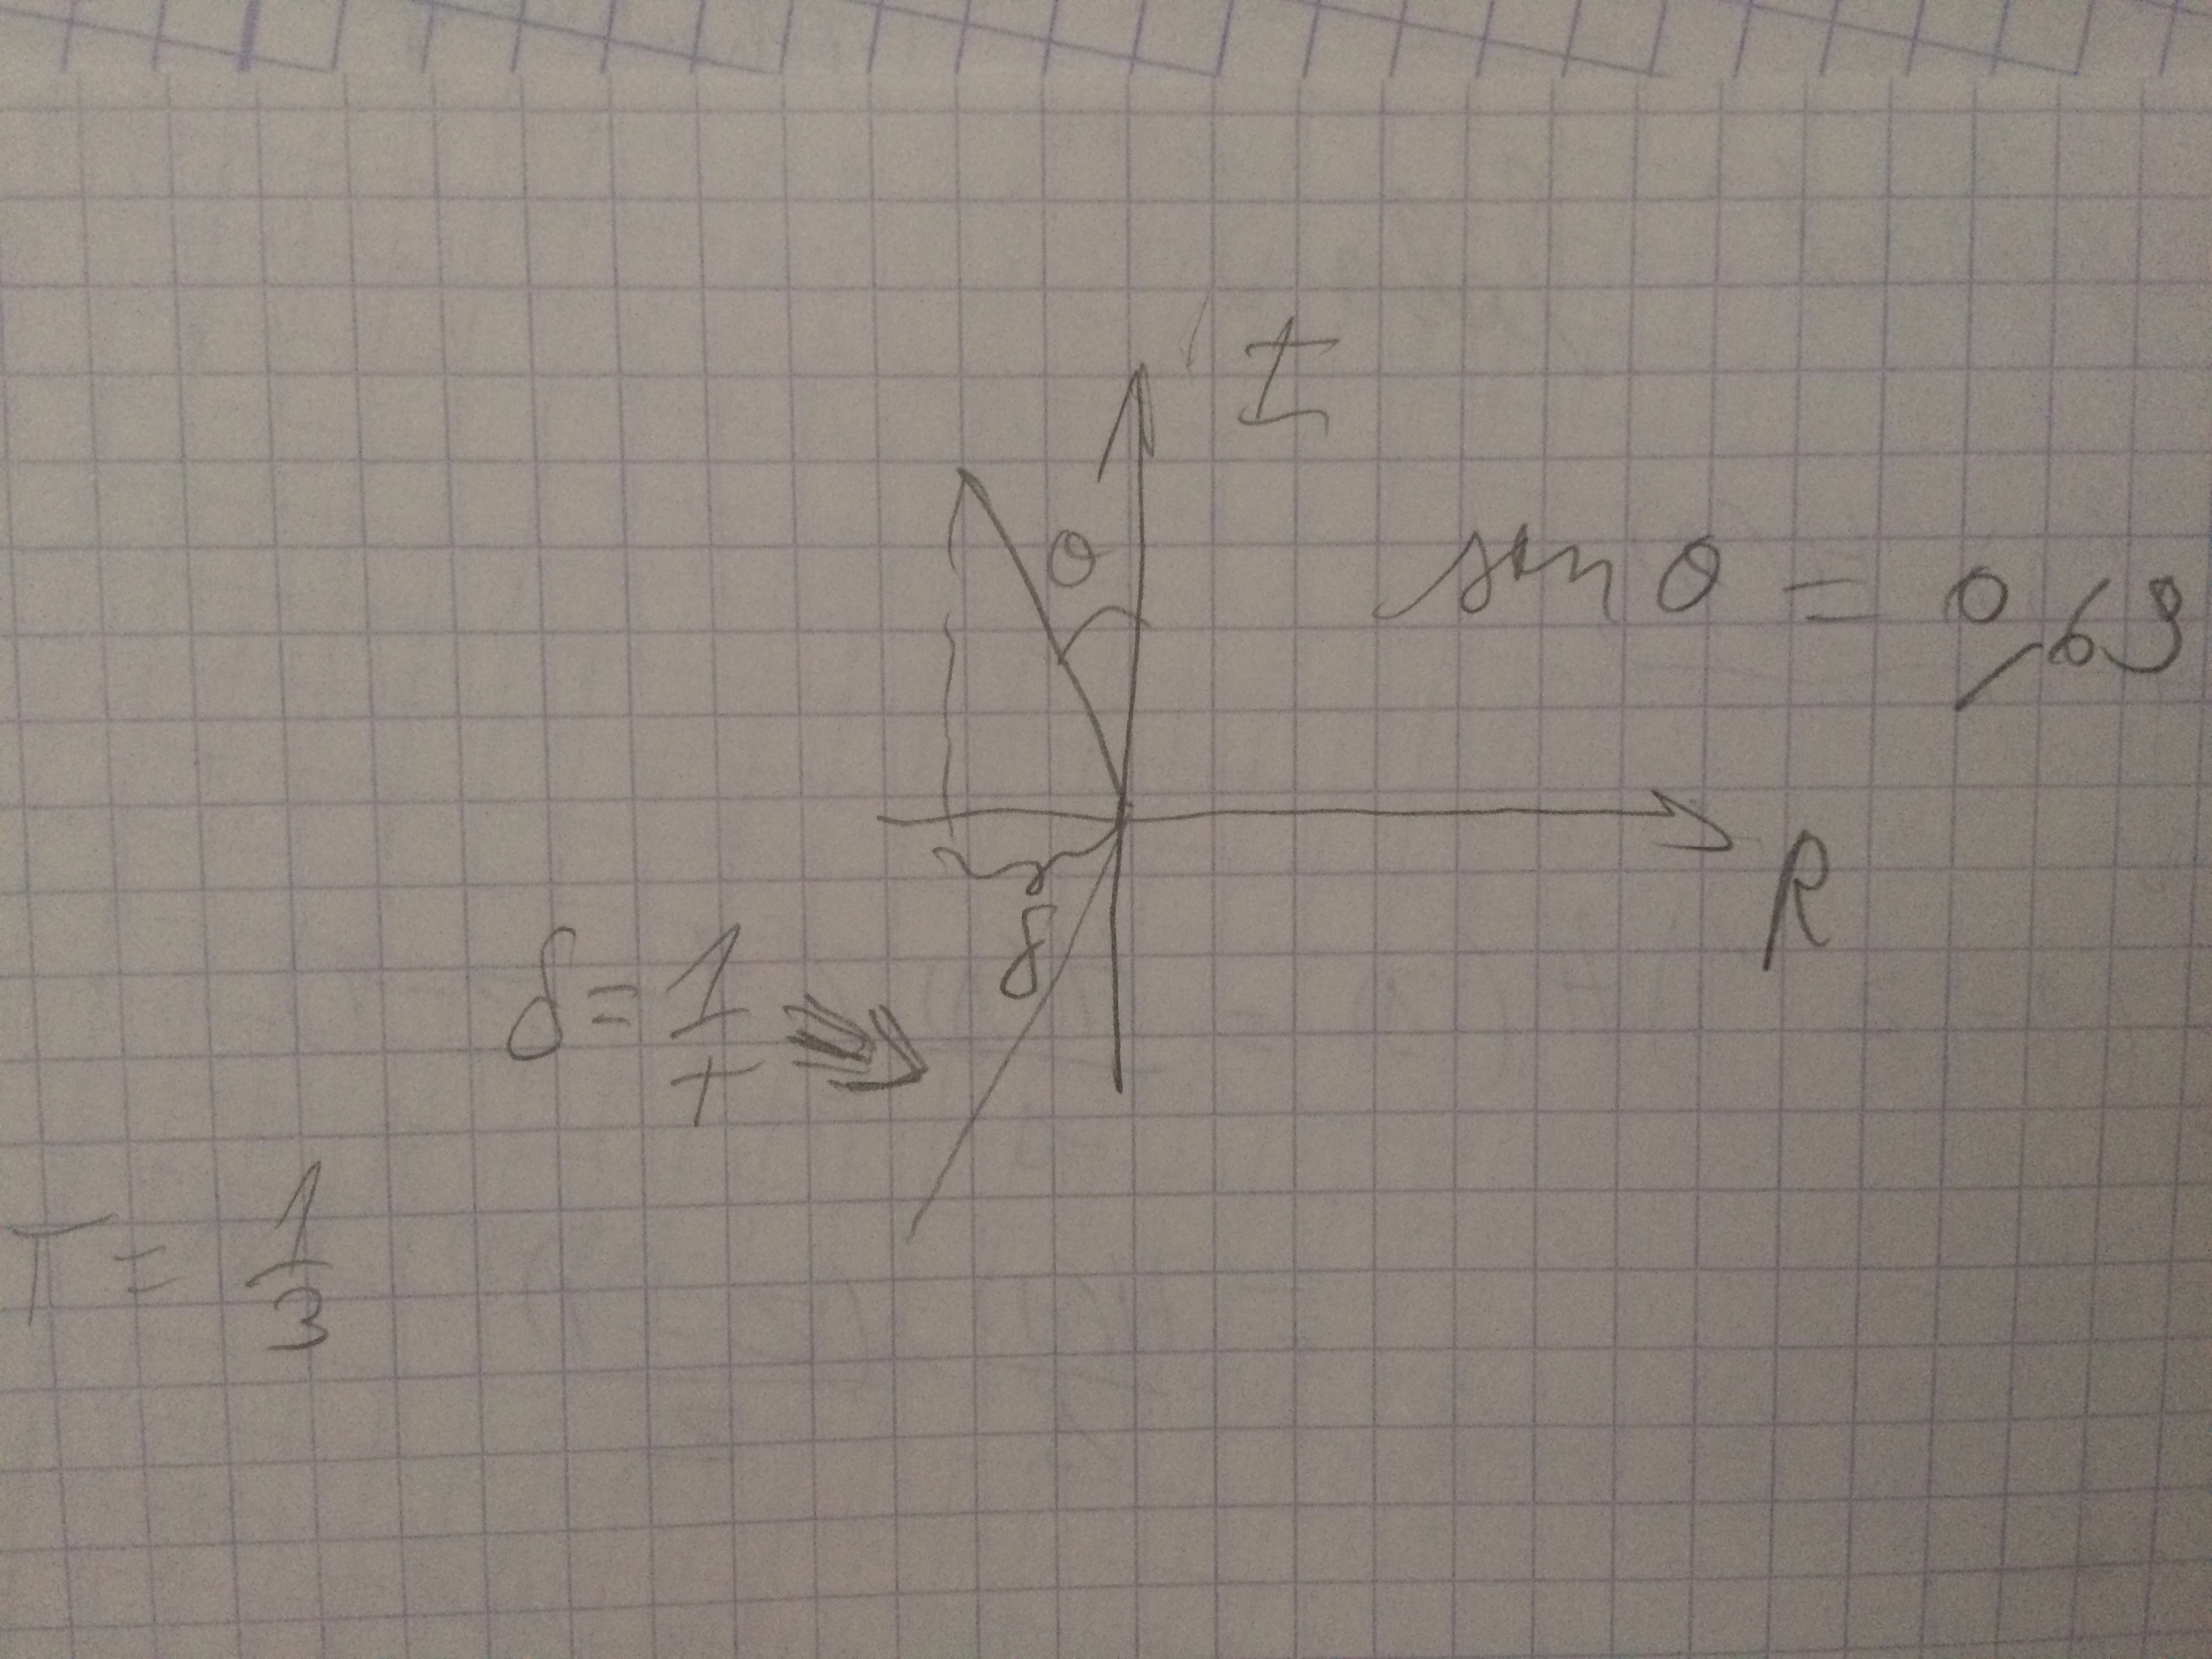
\includegraphics[scale=0.1]{images/IMG_1681.jpg}
	\caption{Temps de réponse.}
	\label{fig:temps-de-reponse}
\end{figure}

Nous pouvons également faire la synthèse du régulateur.
Nous savons que $H_s(Z)$ est sous la forme :
\begin{equation}
	H_s(Z) = \frac{\dots}{(Z-P_{d1})(Z-P_{d2})}
\end{equation}
Nous cherchons à trouver les valeurs de $P_{d1}$ et $P_{d2}$.
Nous allons les trouver par équivalences avec $F(Z)$, la transmittance en boucle fermée.
\begin{equation}
	F(Z) = \frac{k\,(Z-n)}{(Z-1)^2+k\,(Z-n)}
\end{equation}

\begin{equation}
	\begin{cases}
		k = 2-P_{d1}-P_{d2} \\[2mm]
		n = \frac{(1-P_{d1}P_{d2})}{k}
	\end{cases}
	\label{eqn:equivalence}
\end{equation}

En utilisant la fonction \texttt{dtr2ord2o.m} fournie, nous avons pu générer la transmisttance d'un système continu du second ordre répondant aux spécifications.
Nous avons pu extraire les valeurs $P_{d1}$ et $P_{d2}$ de cette transmittance, et par résolution du système~\ref{eqn:equivalence} nous avons obtenu la transmittance du système à synthétiser en boucle fermée.

\section{Conclusion}
Après avoir rentré la fonction de transfert et son régulateur dans Simulink, nous avons pu simuler son action correctrice.
Les résultats sont observables sur les figures \ref{fig:action-correctrice} et \ref{fig:systeme-complet}.
L'effet de l'échantillonnage se fait clairement ressentir sur l'action correctrice.
Nous espérions, des dires du professeur, observer des oscillations sur la réaction du système en boucle fermée mais nous n'observons rien de tel.
Malgré nos chipotages dans les paramètres de simulink, nous ne sommes pas arrivé à mettre en avant de phénomène.

\begin{figure}[!t]
	\centering
	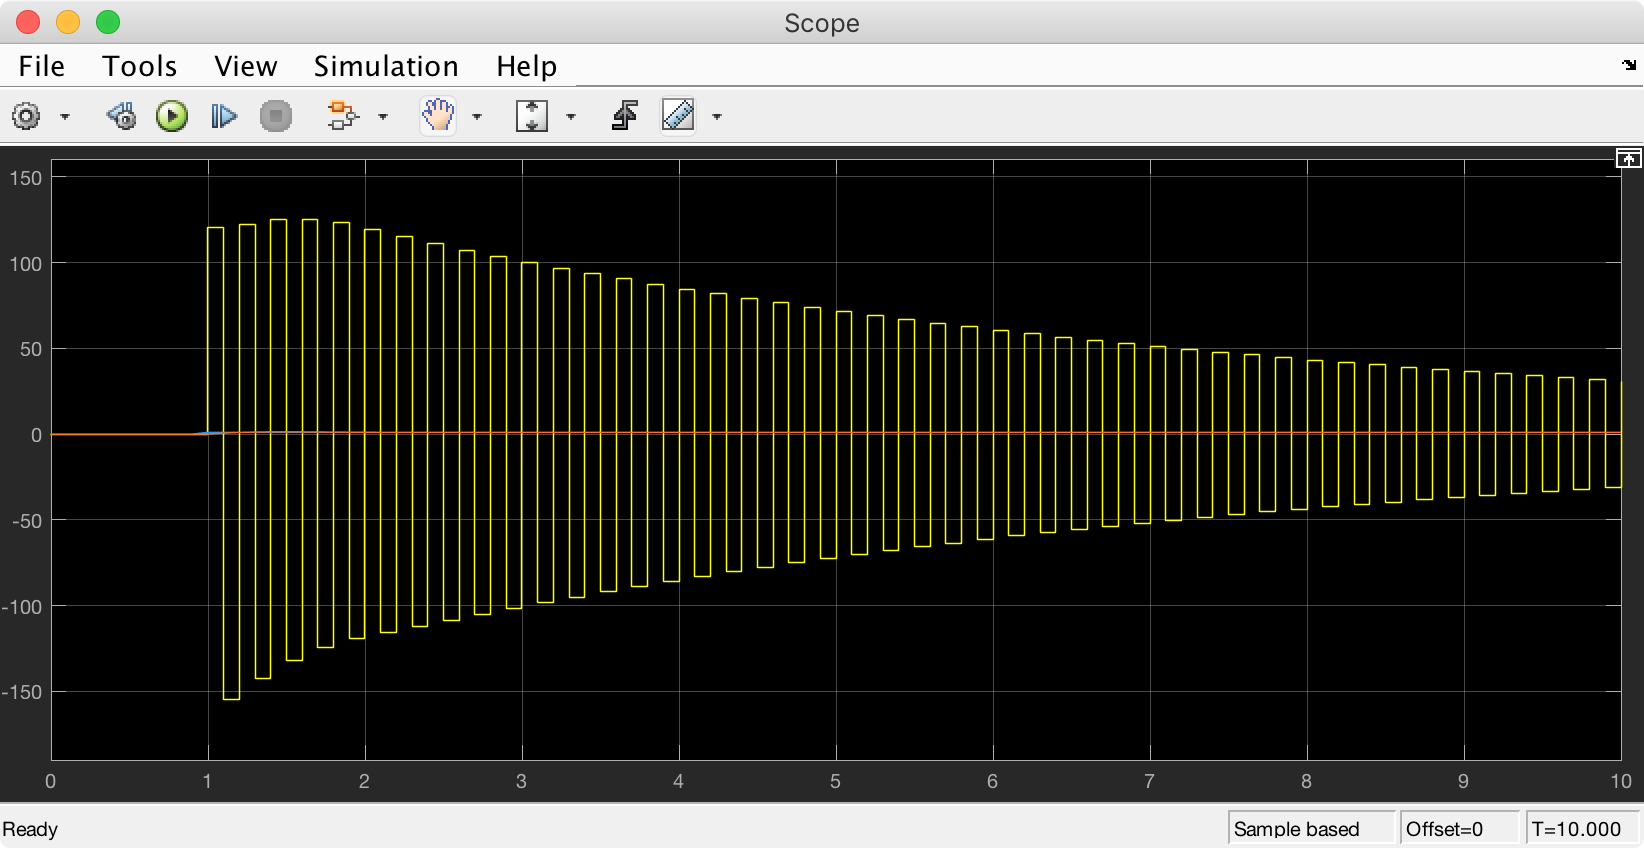
\includegraphics[width=0.9\textwidth]{images/action-reaction.png}
	\caption{Effet de l'action correctrice du régulateur discret.}
	\label{fig:action-correctrice}
\end{figure}

\begin{figure}[!ht]
	\centering
	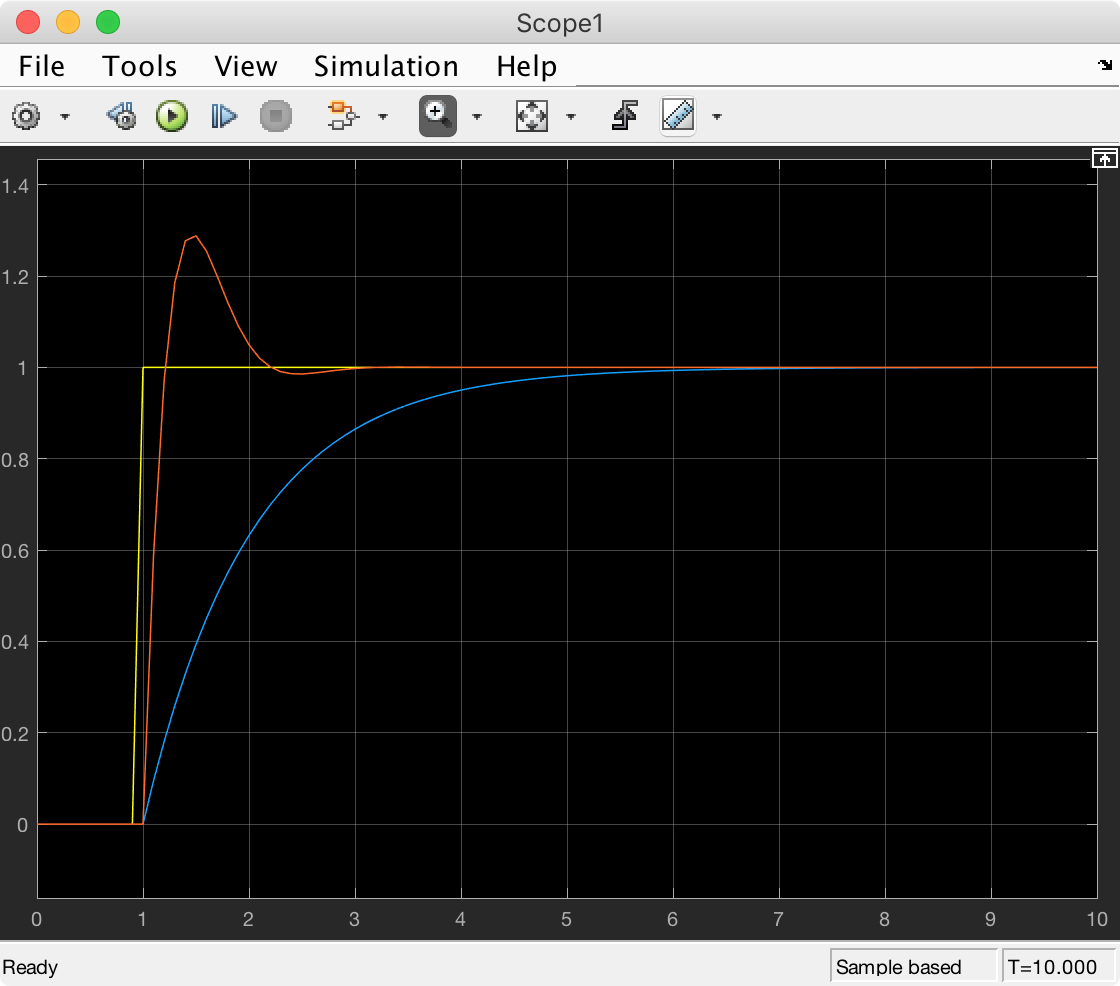
\includegraphics[width=0.8\textwidth]{images/system-complet.png}
	\caption{Réaction du système en boucle fermée à un échelon unitaire.}
	\label{fig:systeme-complet}
\end{figure}
